\section{Inversion am Kreis}\label{kapitel:Inversion}
Inversion am Kreis ist eine geometrische Transformation. Die \enquote{klassischen} geometrischen Transformationen, wie Drehungen, Spiegelungen oder zentrische Streckungen, sind häufig nützliche Hilfsmittel. Allerdings bringt es wenig, sie direkt auf eine Aufgabenstellung anzuwenden: Wenn ihr eine Aufgabe um einen Punkt dreht, erhaltet ihr die gleiche Aufgabe zurück. Mit der Inversion verhält sich das anders: Wenn ihr eine Aufgabe an einem Kreis invertiert, erhaltet ihr im Allgemeinen eine völlig andere (aber äquivalente!) Aufgabe. Und wenn ihr euch geschickt anstellt, ist die neue Aufgabe einfacher als die alte!

Wir werden zuerst die Theorie besprechen und dann an mehreren Olympiadeaufgaben demonstrieren, wie Inversion am Kreis effektiv eingesetzt werden kann.

\subsection*{Formale Eigenschaften der Inversion}
\begin{definition}
	Sei $\Omega$ ein Kreis mit Mittelpunkt~$O$ und Radius~$r$. Die \emph{Inversion an~$\Omega$} ist diejenige Abbildung der Ebene (ohne~$O$) auf sich selbst, die einen beliebigen Punkt $A\neq O$ auf denjenigen Punkt~$A'$ auf dem Strahl~$\overrightarrow{OA}$ schickt, für den $\abs{OA}\cdot \abs{OA'}=r^2$ gilt.
\end{definition}

\begin{satzmitnamen}[Eigenschaften der Inversion]
	Sei $\iota$ die Inversion an~$\Omega$.
	\begin{enumerate}
		\item \label{itm:Involution}
		Für jeden Punkt $A\neq O$ ist $\iota(\iota(A))=A$. Mit anderen Worten: Die zweimalige Hintereinanderausführung $\iota\circ\iota$ ist die Identität.
		\item \label{itm:Vertauschen}
		Punkte im Inneren von~$\Omega$ werden durch~$\iota$ auf Punkte außerhalb von~$\Omega$ geschickt und umgekehrt. Punkte auf~$\Omega$ bleiben unter~$\iota$ fixiert.
		\item \label{itm:Winkel}
		Seien $A,B\neq O$ zwei beliebige Punkte und $A'$,~$B'$ ihre Bilder unter~$\iota$. Dann gilt $\winkel OAB=\winkel A'B'O$ und $\winkel ABO=\winkel OA'B'$. %Insbesondere sind die Dreiecke $OAB$ und $OA'B'$ gegensinning ähnlich.
		\item \label{itm:GeradeGerade}
		Geraden, die durch~$O$ verlaufen, werden von~$\iota$ auf sich selbst abgebildet.
		\item \label{itm:GeradeKreis}
		Geraden, die nicht durch~$O$ verlaufen, werden durch~$\iota$ auf Kreise abgebildet, die durch~$O$ verlaufen, und umgekehrt.
		\item \label{itm:KreisKreis}
		Kreise, die nicht durch~$O$ verlaufen, werden durch~$\iota$ wieder auf Kreise abgebildet, die nicht durch~$O$ verlaufen.
	\end{enumerate}
\end{satzmitnamen}

Um Eigenschaft~\ref{itm:GeradeKreis} besser zu verstehen, ist es hilfreich, einen \enquote{unendlich weit entfernten Punkt}~$\infty$ zur Euklidischen Ebene hinzuzufügen und $\iota(O)\coloneqq \infty$, $\iota(\infty)\coloneqq O$ zu definieren. Wir betrachten dann Geraden und Kreise als \emph{verallgemeinerte Kreise}: Ein verallgemeinerter Kreis ist eine Gerade, wenn er durch den unendlich weit entfernten Punkt~$\infty$ geht, sonst ist er ein normaler Kreis. Damit werden die Eigenschaften \ref{itm:GeradeKreis} und~\ref{itm:KreisKreis} zu einem Spezialfall der folgenden Eigenschaft:
\begin{enumerate}[label={$(\alph*')$}, ref={$(\alph*')$}, start=6]\itshape
	\item \label{itm:veralgKreis}
	Verallgemeinerte Kreise werden durch $\iota$ auf verallgemeinerte Kreise abgebildet.
\end{enumerate}
Aus Eigenschaft~\ref{itm:veralgKreis} folgt nämlich, dass $\iota$ verallgemeinerte Kreise durch~$O$ auf verallgemeinerte Kreise durch $\iota(O)=\infty$ abbildet und umgekehrt; das liefert uns genau Eigenschaft~\ref{itm:GeradeKreis}. Und verallgemeinerte Kreise, die weder durch~$O$ noch durch~$\infty$ gehen, werden auch nach der Inversion nicht durch~$O$ oder~$\infty$ gehen, sodass wir Eigenschaft~\ref{itm:KreisKreis} zurückbekommen.

Für verallgemeinerte Kreise lässt sich ein \emph{Schnittwinkel} definieren. Für zwei Geraden ist der Schnittwinkel wie üblich definiert: Die beiden Geraden spannen zwei Paare von Scheitelwinkeln auf, sodass wir zwei Werte erhalten, die sich zu~$180^\circ$ ergänzen; der Schnittwinkel ist dann der kleinere der beiden Werte (sodass der Schnittwinkel immer zwischen $0^\circ$~und~$90^\circ$ liegt). Der Schnittwinkel zweier Kreise ist definiert als der Schnittwinkel der Tangenten in einem Schnittpunkt der Kreise (sofern mindestens ein Schnittpunkt existiert; ansonsten ist der Schnittwinkel undefiniert). Analog definieren wir den Schnittwinkel zwischen einer Gerade und einem Kreis. Mit dieser Definition können wir zwei weitere Eigenschaften der Inversion formulieren:
\begin{enumerate}[resume]\itshape
	\item \label{itm:Schnitt}
	Wenn sich zwei verallgemeinerte Kreise im Winkel~$\varphi$ schneiden \embrace{wobei $0^\circ\leqslant \varphi\leqslant 90^\circ$}, dann schneiden sich auch ihre Bilder unter~$\iota$ im Winkel~$\varphi$.
	\item \label{itm:Schnitt90}
	Verallgemeinerte Kreise, die $\Omega$ im Winkel~$90^\circ$ schneiden, werden durch $\iota$ auf sich selbst abgebildet.
\end{enumerate}

Zwei Warnungen, bevor wir die Eigenschaften beweisen:
\begin{itemize}[\Warnung]
	\item In vielen Texten wird davon gesprochen, dass Inversion \emph{winkeltreu} ist. Damit ist Eigenschaft~\ref{itm:Schnitt} gemeint. Es folgt jedoch \emph{nicht}, dass $\winkel BAC=\winkel B'A'C'$ für beliebige drei Punkte $A$,~$B$ und~$C$ sowie ihre Bildpunkte $A'$,~$B'$ und~$C'$ gilt.
	\item Eigenschaft~\ref{itm:KreisKreis} besagt nur, dass Inversion Kreise, die nicht durch $O$ verlaufen, auf ebensolche Kreise abbildet. Es folgt \emph{nicht}, dass auch die Mittelpunkte aufeinander abgebildet werden.
\end{itemize}

\begin{proof}[Beweis der Eigenschaften]
	Die Eigenschaften~\ref{itm:Involution},~\ref{itm:Vertauschen} und~\ref{itm:GeradeGerade} folgen direkt aus der Definition.
	
	\emph{Eigenschaft~\ref{itm:Winkel}.} Wir bemerken zuerst, dass $\winkel AOB=\winkel A'OB'$ gilt, denn $A'$~und~$B'$ liegen auf den Strahlen $\overrightarrow{OA}$ und~$\overrightarrow{OB}$. Ferner ist
	\begin{equation*}
		\frac{\abs{OA'}}{\abs{OB'}}=\frac{r^2\!/\abs{OA}}{r^2\!/\abs{OB}}=\frac{\abs{OB}}{\abs{OA}}\,.
	\end{equation*}
	Nach dem Ähnlichkeitssatz~\emph{sws} sind die Dreiecke $OAB$ und $OA'B'$ also gegensinnig ähnlich. Die behauptete Winkelgleichheit in Eigenschaft~\ref{itm:Winkel} folgt unmittelbar.
	\begin{figure}[ht]
		\centering
		\begin{tabularx}{\textwidth}{X c X c X}
			& 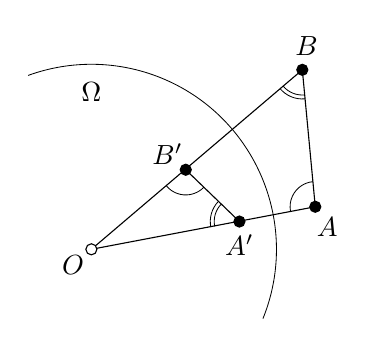
\begin{tikzpicture}[x=2.35cm,y=2.35cm]
				\draw[line width=0.3] (-22:1) arc (-22:110:1);
				\coordinate (O) at (0,0);
				\coordinate (A) at (1.21,0.23);
				\coordinate (A1) at (0.8,0.15);
				\coordinate (B) at (1.14,0.97);
				\coordinate (B1) at (0.51,0.43);
				\draw (O) to (A);
				\draw (O) to (B);
				\draw (A) to (B);
				\draw (A1) to (B1);
				\draw[line width=0.3, shift={(A)}] (95.1:0.32cm) arc (95.1:190.9:0.32cm);
				\draw[line width=0.3, shift={(B1)}] (220.29:0.32cm) arc (220.29:316.09:0.32cm);
				\draw[line width=0.3, shift={(B)}] (220.29:0.32cm) arc (220.29:275.1:0.32cm);
				\draw[line width=0.3, shift={(B)}] (220.29:0.37cm) arc (220.29:275.1:0.37cm);
				\draw[line width=0.3, shift={(A1)}] (136.09:0.32cm) arc (136.09:190.9:0.32cm);
				\draw[line width=0.3, shift={(A1)}] (136.09:0.37cm) arc (136.09:190.9:0.37cm);
				\draw[fill=white] (O) circle (2pt) node[shift={(220:2ex)}] {$O$};
				\draw[fill=black] (A) circle (2pt) node[shift={(-60:2ex)}] {$A$};
				\draw[fill=black] (A1) circle (2pt) node[shift={(-90:2ex)}] {$A'$};
				\draw[fill=black] (B) circle (2pt) node[shift={(80:2ex)}] {$B$};
				\draw[fill=black] (B1) circle (2pt) node[shift={(140:2ex)}] {$B'$};
				\node at (0,0.85) {$\Omega$};
			\end{tikzpicture} & & 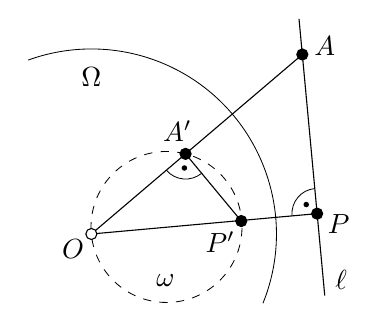
\begin{tikzpicture}[x=2.35cm,y=2.35cm]
				\draw[line width=0.3] (-22:1) arc (-22:110:1);
				\coordinate (O) at (0,0);
				\draw[line width=0.3,dashed] (0.406,0.038) circle (0.408);
				\coordinate (P) at (1.22,0.11);
				\coordinate (P1) at (0.81,0.07);
				\coordinate (A) at (1.14,0.97);
				\coordinate (A1) at (0.509,0.433);
				\draw (O) to (A);
				\draw (O) to (P);
				\draw[shorten <=-3ex,shorten >=-6.9ex] (A) to (P);
				\draw (A1) to (P1);
				\draw[line width=0.3, shift={(P)}] (95.1:0.32cm) arc (95.1:185.1:0.32cm);
				\fill[shift={(P)}] (140.1:0.18cm) circle (1pt);
				\draw[line width=0.3, shift={(A1)}] (220.29:0.32cm) arc (220.29:310.29:0.32cm);
				\fill[shift={(A1)}] (265.29:0.18cm) circle (1pt);
				\draw[fill=white] (O) circle (2pt) node[shift={(220:2ex)}] {$O$};
				\draw[fill=black] (P) circle (2pt) node[shift={(-25:2ex)}] {$P$};
				\draw[fill=black] (P1) circle (2pt) node[shift={(-135:2.5ex)}] {$P'$};
				\draw[fill=black] (A) circle (2pt) node[shift={(20:2ex)}] {$A$};
				\draw[fill=black] (A1) circle (2pt) node[shift={(110:2ex)}] {$A'$};
				\node at (0,0.85) {$\Omega$};
				\node at (0.4,-0.25) {$\omega$};
				\node at (1.35,-0.25) {$\ell$};
			\end{tikzpicture} & \\\addlinespace
			& Eigenschaft~\ref{itm:Winkel} & & Eigenschaft~\ref{itm:GeradeKreis} & 
		\end{tabularx}
	\end{figure}
	
	\emph{Eigenschaft~\ref{itm:GeradeKreis}.} Betrachte eine Gerade~$\ell$, die nicht durch~$O$ verläuft. Sei $P$ der Lotfußpunkt von~$O$ auf~$\ell$. Seien $P'$~und~$\ell'$ die Bilder von $P$~und~$\ell$ unter~$\iota$. Wir werden zeigen, dass $\ell'$ der Kreis~$\omega$ mit Durchmesser~$\overline{OP'}$ ist. Für jeden Punkt~$A$ auf~$\ell$ ist $\winkel APO=90^\circ$. Aus Eigenschaft~\ref{itm:Winkel} folgt $\winkel OA'P'=90^\circ$. Nach dem Satz von Thales liegt $A'$ somit auf~$\omega$. Damit ist gezeigt, dass $\ell'$ in~$\omega$ enthalten ist. Umgekehrt zeigt das gleiche Argument, dass für jeden Punkt~$B$ auf~$\omega$ der Bildpunkt~$\iota(B)$ auf~$\ell$ liegen muss (das stimmt auch für $B=O$, denn dann ist $\iota(B)=\infty$). Wegen $\iota(\iota(B))=B$ folgt, dass $\ell'$ jeden Punkt auf~$\omega$ enthält. Also wird $\ell$ unter der Inversion tatsächlich bijektiv auf~$\omega$ abgebildet. Damit ist gezeigt, dass $\iota$ Geraden auf Kreise durch~$O$ abbildet. Die umgekehrte Aussage folgt aus dem gleichen Argument, oder alternativ aus Eigenschaft~\ref{itm:Involution}.
	
	\emph{Eigenschaft~\ref{itm:KreisKreis}.} Sei $\omega$ ein Kreis, der nicht durch~$O$ verläuft. Die Gerade, die durch~$O$ und den Mittelpunkt von~$\omega$ verläuft, schneide $\omega$ in den Punkten $A$~und~$B$, sodass $\overline{AB}$ ein Durchmesser von~$\omega$ ist. Wir nehmen im Folgenden an, dass $A$~und~$B$ auf der gleichen Seite von~$O$ liegen (sodass $O$ außerhalb von~$\omega$ liegt); der andere Fall geht analog. Seien $\omega'$, $A'$~und~$B'$ die jeweiligen Bilder unter~$\iota$. Wir werden zeigen, dass $\omega'$ ein Kreis mit Durchmesser~$\overline{A'B'}$ ist. Dazu betrachte einen beliebigen Punkt~$C$ auf~$\omega$ und seinen Bildpunkt $C'=\iota(C)$. Nach Thales gilt $\winkel ACB=90^\circ$ und nach Außenwinkelsatz im Dreieck $ABC$ ist $\winkel CAO=90^\circ+\winkel CBO$. Aus Eigenschaft~\ref{itm:Winkel} folgt $\winkel OC'B'=\winkel CBO$ und $\winkel OC'A'=\winkel CAO=90^\circ+\winkel CBO$. Also ist
	\begin{equation*}
		\winkel B'C'A'=\winkel OC'A'-\winkel OC'B'= \parens{90^\circ+\winkel CBO}-\winkel CBO=90^\circ\,.
	\end{equation*}
	Aus der Umkehrung des Satzes von Thales folgt, dass $C'$ auf dem Kreis mit Durchmesser~$\overline{A'B'}$ liegt. Also ist $\omega'$ in diesem Kreis enthalten. Analog zu Eigenschaft~\ref{itm:GeradeKreis} argumentierten wir, dass $\omega'$ tatsächlich mit diesem Kreis identisch sein muss. Also ist $\omega'$ in der Tat ein Kreis.
	
	\begin{figure}[ht]
		\centering
		\begin{tabularx}{\textwidth}{X c X c X}
			& 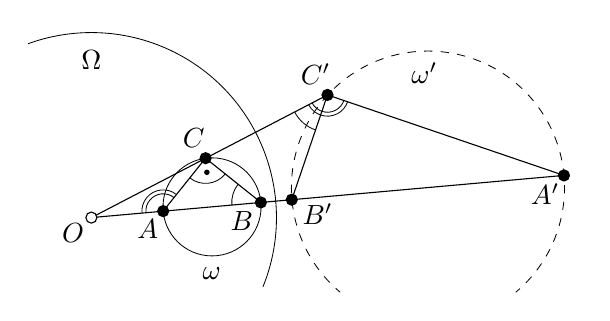
\begin{tikzpicture}[x=2.35cm,y=2.35cm]
				\draw[line width=0.3] (-22:1) arc (-22:110:1);
				\draw[line width=0.3] (0.652,0.058) circle (0.265);
				\draw[line width=0.3,dashed,shift={(1.819,0.162)}, dash phase=1] (-50:0.738) arc (-50:230:0.738);
				\coordinate (O) at (0,0);
				\coordinate (A) at (0.388,0.035);
				\coordinate (A1) at (2.554,0.228);
				\coordinate (B) at (0.916,0.082);
				\coordinate (B1) at (1.083,0.097);
				\coordinate (C) at (0.617,0.321);
				\coordinate (C1) at (1.276,0.663);
				\draw (O) to (A1);
				\draw (O) to (C1);
				\draw (A) to (C);
				\draw (B) to (C);
				\draw (B1) to (C1);
				\draw (A1) to (C1);
				\draw [line width=0.3,shift={(A)}] (51.358:0.27cm) arc (51.358:185.104:0.27cm);
				\draw [line width=0.3,shift={(A)}] (51.358:0.22cm) arc (51.358:185.104:0.22cm);
				\draw [line width=0.3,shift={(C)}] (231.358:0.32cm) arc (231.358:321.358:0.32cm);
				\fill [line width=0.3,shift={(C)}] (275.358:0.18cm) circle (1pt);
				\draw [line width=0.3,shift={(B)}] (141.358:0.37cm) arc (141.358:185.104:0.37cm);
				\draw [line width=0.3,shift={(C1)}] (207.457:0.27cm) arc (207.457:341.203:0.27cm);
				\draw [line width=0.3,shift={(C1)}] (207.457:0.47cm) arc (207.457:251.203:0.47cm);
				\draw [line width=0.3,shift={(C1)}] (207.457:0.22cm) arc (207.457:341.203:0.22cm);
				\draw[fill=white] (O) circle (2pt) node[shift={(220:2ex)}] {$O$};
				\draw[fill=black] (A) circle (2pt) node[shift={(230:2ex)}] {$A$};
				\draw[fill=black] (A1) circle (2pt) node[shift={(225:2.25ex)}] {$A'$};
				\draw[fill=black] (B) circle (2pt) node[shift={(225:2.25ex)}] {$B$};
				\draw[fill=black] (B1) circle (2pt) node[shift={(-30:2.5ex)}] {$B'$};
				\draw[fill=black] (C) circle (2pt) node[shift={(120:2ex)}] {$C$};
				\draw[fill=black] (C1) circle (2pt) node[shift={(120:2ex)}] {$C'$};
				\node at (0,0.85) {$\Omega$};
				\node at (0.65,-0.3) {$\omega$};
				\node at (1.8,0.78) {$\omega'$};
			\end{tikzpicture} & & 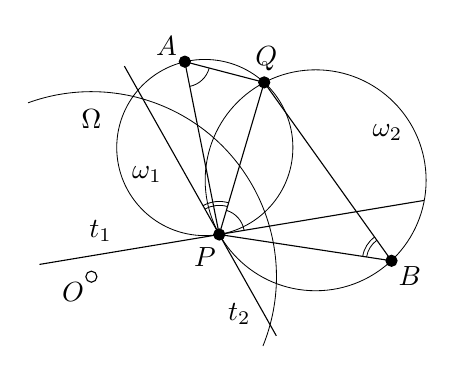
\begin{tikzpicture}[x=2.35cm,y=2.35cm]
				\draw[line width=0.3] (-22:1) arc (-22:110:1);
				\draw[line width=0.3] (0.613,0.698) circle (0.476);
				\draw[line width=0.3] (1.212,0.521) circle (0.597);
				\coordinate (O) at (0,0);
				\coordinate (A) at (0.505,1.162);
				\coordinate (P) at (0.691,0.228);
				\coordinate (Q) at (0.934,1.05);
				\coordinate (B) at (1.622,0.086);
				\draw (P) to (Q);
				\draw (A) to (P) to (B) to (Q) to cycle;
				\draw[shorten <=-2.5em,shorten >=-4.2em] (0.362,0.812) to (P);
				\draw[shorten <=-3em,shorten >=-7.5em] (0.162,0.14) to (P);
				\draw [line width=0.3,shift={(P)}] (9.412:0.32cm) arc (9.412:73.511:0.32cm);
				\draw [line width=0.3,shift={(P)}] (73.511:0.37cm) arc (73.511:119.337:0.37cm);
				\draw [line width=0.3,shift={(P)}] (73.511:0.42cm) arc (73.511:119.337:0.42cm);
				\draw [line width=0.3,shift={(A)}] (281.23:0.32cm) arc (281.23:345.328:0.32cm);
				\draw [line width=0.3,shift={(B)}] (125.524:0.32cm) arc (125.524:171.367:0.32cm);
				\draw [line width=0.3,shift={(B)}] (125.524:0.37cm) arc (125.524:171.367:0.37cm);
				\draw[fill=white] (O) circle (2pt) node[shift={(220:2ex)}] {$O$};
				\draw[fill=black] (A) circle (2pt) node[shift={(140:2ex)}] {$A$};
				\draw[fill=black] (B) circle (2pt) node[shift={(-40:2ex)}] {$B$};
				\draw[fill=black] (P) circle (2pt) node[shift={(238:2.25ex)}] {$P$};
				\draw[fill=black] (Q) circle (2pt) node[shift={(85:2ex)}] {$Q$};
				\node at (0,0.85) {$\Omega$};
				\node at (0.3,0.55) {$\omega_1$};
				\node at (1.6,0.78) {$\omega_2$};
				\node at (0.05,0.245) {$t_1$};
				\node at (0.8,-0.2) {$t_2$};
			\end{tikzpicture} & \\\addlinespace
			& Eigenschaft~6 & & Eigenschaft~7 & 
		\end{tabularx}
	\end{figure}
	
	\emph{Eigenschaft~\ref{itm:veralgKreis}.} Bei dieser Eigenschaft sind mehrere Fälle zu unterscheiden, je nachdem, welche der verallgemeinerten Kreise durch $O$ oder~$\infty$ verlaufen. Wir werden nur den (schwierigsten) Fall betrachten, in dem wir es mit zwei Kreisen zu tun haben, die nicht durch~$O$ (und nicht durch~$\infty$) verlaufen, und überlassen es euch als Übungsaufgabe, die Argumente auf die anderen Fälle zu übertragen. Ferner ergeben sich in dem betrachteten Fall je nach Lage der Kreise mehrere Unterfälle. Wir werden der Einfachheit halber nur einen Lagefall betrachten. Für diejenigen unter euch, die bereits mit orientierten Winkeln modulo~$180^\circ$ vertraut sind, ist der Beweis so formuliert, dass er unter Verwendung von orientierten Winkeln modulo~$180^\circ$ für alle Lagefälle gültig ist.
	
	Betrachte also zwei Kreise $\omega_1$~und~$\omega_2$, die sich in den Punkten $P$~und~$Q$ im Winkel~$\varphi$ schneiden. Wähle ferner einen Punkt~$A$ auf~$\omega_1$ und einen Punkt~$B$ auf~$\omega_2$, sodass $A$~außerhalb von~$\omega_2$ und $B$~außerhalb von~$\omega_1$ liegt. Die Bilder unter~$\iota$ werden mit $A'$,~$B'$, $P'$, $Q'$, $\omega_1'$ und~$\omega_2'$ bezeichnet. Seien $t_1$~und~$t_2$ die Tangenten an $\omega_1$~und~$\omega_2$ in~$P$. Nach dem Sehnen-Tangentenwinkelsatz ist $\winkel (t_1,PQ)=\winkel PAQ$ und $\winkel (PQ,t_2)=\winkel QBP$. Folglich schneiden sich $t_1$~und~$t_2$ im Winkel $\winkel(t_1,PQ)+\winkel (PQ,t_2)=\winkel PAQ+\winkel QBP$. Das heißt allerdings nicht unbedingt, dass $\winkel PAQ+\winkel QBP=\varphi$ gelten muss: Dadurch, dass wir für Schnittwinkel stets $0^\circ\leqslant \varphi\leqslant 90^\circ$ fordern, kann $\winkel PAQ+\winkel QBP$ auch die Werte $180^\circ-\varphi$, $180^\circ+\varphi$ oder sogar $360^\circ-\varphi$ annehmen. In jedem Fall ist es aber ausreichend, $\winkel PAQ+\winkel QBP=\winkel Q'A'P'+\winkel P'B'Q'$ zu zeigen, denn wir können das gleiche Argument für $\omega_1'$~und~$\omega_2'$ anwenden. Dazu erinnern wir uns an Eigenschaft~\ref{itm:Winkel} und erhalten $\winkel Q'A'P'=\winkel OA'P'-\winkel OA'Q'=\winkel APO-\winkel AQO$ und analog $\winkel P'B'Q'=\winkel OPB-\winkel OQB$. Sodann rechnen wir
	\begin{align*}
		\winkel Q'A'P'+\winkel P'B'Q'&=\parens{\winkel APO+\winkel OPB}-\parens{\winkel AQO+\winkel OQB}\\
		&=360^\circ-\winkel BPA-\winkel AQB\\
		&=\winkel PAQ+\winkel QBP\,.
	\end{align*}
	Im zweiten Schritt haben wir benutzt, dass sich $\winkel APO$, $\winkel OPB$ und $\winkel BPA$ zu~$360^\circ$ ergänzen. Im dritten Schritt haben wir die Innenwinkelsumme im Viereck $APBQ$ eingesetzt. Das beendet den Beweis von Eigenschaft~\ref{itm:veralgKreis}.
	
	\emph{Eigenschaft~\ref{itm:Schnitt90}.} Sei $\omega$ ein verallgemeinerter Kreis, der $\Omega$ im Winkel~$90^\circ$ schneidet, und seien $A$~und~$B$ die beiden Schnittpunkte. Die Punkte $A$~und~$B$ werden durch~$\iota$ auf sich selbst abgebildet. Nach Eigenschaft~\ref{itm:Schnitt} ist das Bild von~$\omega$ also wiederum ein verallgemeinerter Kreis durch $A$~und~$B$, der $\Omega$ im Winkel~$90^\circ$ schneidet. Für je zwei Punkte $A$~und~$B$ gibt es aber genau einen verallgemeinerten Kreis durch $A$~und~$B$, der $\Omega$ im Winkel~$90^\circ$ schneidet (wenn $A$~und~$B$ diametral gegenüberliegen, ist dieser verallgemeinerte Kreis eine Gerade, ansonsten ein echter Kreis). Also muss $\omega$ auf sich selbst abgebildet werden.
\end{proof}

\subsection*{Strategien, Tipps und Tricks für Inversionslösungen}
Fast immer ist es egal, welchen Radius der Kreis hat, an dem wir invertieren. Wenn im Folgenden die Rede davon ist, dass \emph{an einem Punkt~$O$ invertiert wird}, so ist gemeint, dass wir an einem Kreis um~$O$ mit beliebigem Radius invertieren.
\begin{itemize}
	\item Die wichtigste Eigenschaft der Inversion ist Nummer~\ref{itm:GeradeKreis}, denn sie erlaubt uns, Aufgaben mit Kreisen in Aufgaben mit Geraden zu überführen, die häufig einfacher sind (und dank Eigenschaft~\ref{itm:Involution} ist die neue Aufgabe zur alten äquivalent).
	\item Invertieren an einem Punkt~$O$ lohnt sich besonders dann, wenn viele Kreise und viele Geraden durch~$O$ gehen. Denn so werden möglichst viele Kreise zu Geraden und möglichst wenige Geraden zu Kreisen.
	\item Zwei Kreise (oder ein Kreis und eine Gerade) berühren sich in einem Punkt~$O$ genau dann, wenn ihre Bilder unter Inversion an~$O$ zwei parallele Geraden sind, denn zwei Kreise (oder ein Kreis und eine Gerade) haben genau dann nur den Punkt~$O$ gemeinsam, wenn ihre Bilder unter Inversion an~$O$ nur den Punkt~$\infty$ gemeinsam haben. Wenn ihr also in einer Aufgabe zeigen sollt, dass sich zwei Kreise (oder ein Kreis und eine Gerade) berühren, ist es oft eine gute Idee, am gewünschten Berührpunkt zu invertieren. Dann müsst ihr nur noch zeigen, dass zwei Geraden parallel sind, was wesentlich weniger gruselig aussieht. Siehe dazu die Beispielaufgaben.
	\item Wir haben euch bereits gewarnt, dass Inversion die Mittelpunkte von Kreisen nicht erhält. Trotzdem lässt sich häufig herausfinden, worauf der Mittelpunkt eines Kreises geschickt wird. Wenn zum Beispiel $M$~der Mittelpunkt eines Kreises~$\omega$ ist, der durch das Inversionszentrum~$O$ verläuft, dann betrachte denjenigen Punkt~$P$ auf~$\omega$, für den $\overline{OP}$ ein Durchmesser ist. Dann ist $P'$ der Lotfußpunkt von~$O$ auf die Gerade~$\omega'$. Weil $M$ der Mittelpunkt von~$\overline{OP}$ ist, liegt $M'$ auf der Geraden~$OP'$. Andererseits folgt aus $\abs{OM}=\frac 12\abs{OP}$, dass $\abs{OM'}=2\abs{OP'}$ gelten muss. Also ist $M'$ das Spiegelbild von~$O$ an der Geraden~$\omega'$.
	
	Für allgemeinere Mittelpunkte könnt ihr mit ähnlichen Überlegungen, oder manchmal auch mit Eigenschaft~\ref{itm:Winkel}, herausfinden, worauf diese durch die Inversion geschickt werden.
	\item Streckenlängen bleiben natürlich auch nicht unter Inversion erhalten. Trotzdem gibt es eine relativ einfache Formel. Wenn $A$,~$B$ zwei Punkte sind und $A'$,~$B'$ ihre Bildpunkte unter Inversion an einem Kreis um~$O$ mit Radius~$r$, dann sind nach Eigenschaft~\ref{itm:Winkel} die Dreiecke $OAB$ und $OA'B'$ gegensinning ähnlich. Der Ähnlichkeitsfaktor muss dann $\abs{OA'}/\abs{OB}$ sein, also ist
	\begin{equation*}%\label{eq:Laengenformel}
		\abs{A'B'}=\abs{AB}\cdot \frac{\abs{OA'}}{\abs{OB}}=\abs{AB}\cdot \frac{r^2}{\abs{OA}\cdot\abs{OB}}\,.
	\end{equation*}
	\item Gelegentlich treten in Aufgabenstellungen sehr komische Winkelbedingungen auf. Durch geschickte Inversion könnt ihr dank Eigenschaft~\ref{itm:Winkel} dafür sorgen, dass diese Winkel an anderer Stelle in eurer Skizze auftauchen, und dann könnt ihr vielleicht mehr mit der Winkelbedingung anfangen. Siehe dazu die Beispielaufgaben.
	\item Manchmal sieht eure Skizze nach einer Inversion genauso aus wie vorher. Dann ist eure Aufgabe zwar nicht einfacher geworden, aber aus der Erkenntnis, dass die Aufgabe \enquote{symmetrisch unter Inversion} ist, könnt ihr trotzdem nichttriviale Schlüsse ziehen oder sogar die Aufgabe lösen. Siehe dazu die Beispielaufgaben.
	\item Versteift euch nicht zu sehr auf die invertierte Skizze. Wenn ihr nicht weiter kommt, dann versucht, eure Erkenntnisse aus der invertierten Skizze in die ursprüngliche Skizze zu übersetzen und die ursprüngliche Aufgabe damit zu lösen.
\end{itemize}

\subsection*{Beispielaufgaben}
Nun sollt ihr die Theorie aus den vorherigen Unterabschnitten auf Olympiadeaufgaben anwenden. Am Ende des Kapitels findet ihr Tipps zu den Beispielaufgaben und am Ende des Heftes könnt ihr die Lösungen nachlesen.

Diese Aufgaben sind ziemlich schwierig für die 9.\ Klasse. Bevor ihr in die Tipps oder die Lösungen schaut, solltet ihr euch trotzdem selbstständig überlegen, welche der Punkte als Inversionszentren in Frage kommen, um dafür Intuition zu entwickeln. Versucht außerdem, mithilfe der Eigenschaften~\ref{itm:Involution}--\ref{itm:Schnitt90} herauszufinden, wie eure Skizze nach der Inversion aussehen würde.

\begin{aufgabe*}\label{aufgabe:450943}
	In einem spitzwinkligen Dreieck $ABC$ sei $H$ der Lotfußpunkt von~$C$ auf~$AB$. Ferner seien $P$~und~$Q$ die Lotfußpunkte von~$H$ auf $AC$ und~$BC$. Die Umkreise $\odot AHP$ und $\odot HBQ$ schneiden die Strecke~$\overline{PQ}$ in von $P$~und~$Q$ verschiedenen Punkten $S$~und~$T$. Zeige, dass der Umkreis $\odot HTS$ die Gerade~$AB$ berührt.
\end{aufgabe*}

\begin{aufgabe*}[*]\label{aufgabe:IMO1996}
	Sei $P$ ein Punkt im Inneren eines Dreiecks $ABC$ mit der Eigenschaft $\winkel APB-\winkel ACB=\winkel CPA-\winkel CBA$. Beweise, dass sich die Winkelhalbierende von $\winkel PBA$ und die Winkelhalbierende von $\winkel ACP$ auf der Geraden~$AP$ schneiden.
\end{aufgabe*}

\begin{aufgabe*}[*]\label{aufgabe:521243}
	Gegeben sind zwei Kreise $\omega_1$~und~$\omega_2$, die sich in zwei Punkten schneiden. Einer der Schnittpunkte sei~$Q$. Der Punkt~$P$ liege außerhalb des Kreises~$\omega_1$ auf dem Kreis~$\omega_2$. Dabei sei die Lage von~$P$ so gewählt, dass folgende zwei Bedingungen erfüllt sind:
	\begin{enumerate}[label={$(\Alph*)$},ref={$(\Alph*)$}]
		\item Die Gerade~$PQ$ schneidet den Kreis~$\omega_1$ in einem von~$Q$ verschiedenen Punkt~$X$.
		\item Die Tangente an~$\omega_1$ in~$X$ schneidet $\omega_2$ in zwei Punkten $A$~und~$B$.
	\end{enumerate}
	Der Kreis~$\omega$ verlaufe durch die Punkte $A$~und~$B$ und berühre die Parallele~$\ell$ zu~$AB$ durch~$P$. Beweise, dass sich die Kreise $\omega$~und~$\omega_1$ berühren.
\end{aufgabe*}

\begin{aufgabe*}[*]\label{aufgabe:Ptolemaeus}
	Beweise die Ungleichung von Ptolemäus:
	\begin{satzmitnamen}[Ungleichung von Ptolemäus]
		Für beliebige vier paarweise verschiedene Punkte $A$,~$B$, $C$ und~$D$ in der Ebene gilt stets
		\begin{equation*}
			\abs{AB}\cdot \abs{CD}+\abs{BC}\cdot\abs{DA}\geqslant \abs{AC}\cdot \abs{BD}\,.
		\end{equation*}
		Gleichheit gilt genau dann, wenn $ABCD$ ein konvexes Sehnenviereck ist.
	\end{satzmitnamen}
	(Der Gleichheitsfall dieser Ungleichung ist als \emph{Satz von Ptolemäus} bekannt und häufig nützlich, wenn ihr Streckenlängen in einem Sehnenviereck berechnen wollt.)
\end{aufgabe*}

\subsection*{Weitere Übungsaufgaben}
\begin{aufgabe*}
	Sei $ABC$ ein spitzwinkliges Dreieck mit Umkreismittelpunkt~$O$. Die Umkreismittelpunkte der Dreiecke $AOC$ und $BCO$ werden mit $Q$~und~$R$ bezeichnet. Zeige, dass sich die Umkreise $\odot ABO$ und $\odot QOR$ berühren.
\end{aufgabe*}

\begin{aufgabe*}
	Gegeben sei ein Kreis~$\Omega$. Wir definieren eine unendliche Folge weiterer Kreise
	\begin{wrapfigure}[6]{r}{0.25\textwidth} % Tien: Statt \vspace{-...} soll das nur 6 Zeilen einnehmen
		\centering
		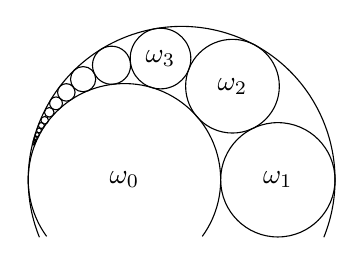
\begin{tikzpicture}
			%\draw (0,0) to (3.896,0);
			%\draw [fill=black] (1.222,0) circle (2pt) node[above] {$\omega_0$};
			%\draw [fill=black] (3.17,0) circle (2pt) node[above] {$\omega_1$};
			\draw [shift={(1.948,0)}] (-22:1.948) arc (-22:202:1.948);
			\draw [shift={(1.222,0)}] node {$\omega_0$} (-36:1.222) arc (-36:216:1.222);
			\pgfresetboundingbox % Tien: Engere bounding box
			\draw (0,0); % Tien: Manuell linker Rand
			\draw (3.17,0) node {$\omega_1$} circle (0.726);
			\draw (2.594,1.189) node {$\omega_2$} circle (0.595);
			\draw (1.68,1.54) node {$\omega_3$} circle (0.385);
			\draw (1.058,1.455)  circle (0.242); %node {$\omega_4$}
			\draw (0.697,1.278) circle (0.16);
			\draw (0.484,1.11) circle (0.111);
			\draw (0.353,0.971) circle (0.081);
			\draw (0.267,0.857) circle (0.061);
			\draw (0.209,0.756) circle (0.048);
			\draw (0.167,0.69) circle (0.038);
			\draw (0.137,0.627) circle (0.031);
			\draw (0.114,0.574) circle (0.026);
			\draw (0.096,0.529) circle (0.022);
			\draw (0.082,0.491) circle (0.019);
			\draw (0.082,0.491) circle (0.019);
			\draw (0.071,0.458) circle (0.016);
		\end{tikzpicture}
	\end{wrapfigure}
	$\omega_0,\omega_1,\omega_2,\dotsc$ wie folgt:
	\begin{itemize}%[label=\textup{\arabic*.},ref=\textup{\arabic*.}]
		\item Die Kreise $\omega_0$~und~$\omega_1$ berühren einander von außen und~$\Omega$ jeweils von innen. Ferner liegen die Mittelpunkte von $\Omega$,~$\omega_0$ und~$\omega_1$ auf einer Geraden.
		\item Für alle $n\geqslant 2$ berührt der Kreis~$\omega_n$ die Kreise $\omega_0$~und~$\omega_{n-1}$ von außen sowie~$\Omega$ von innen.
	\end{itemize}
	Sei $r_n$ der Radius von~$\omega_n$. Berechne $r_n$ in Abhängigkeit von $n$,~$r_0$ und~$r_1$.
\end{aufgabe*}

%\begin{aufgabe*}
%	Sei $ABCD$ ein Trapez mit $AB\parallel CD$. Sei $P$ ein innerer Punkt des Trapezes, für den $\winkel BPC=\winkel DPA$ gilt. Zeige, dass sich die Umkreise $\odot ABP$ und $\odot CDP$ berühren.
%\end{aufgabe*}

\begin{aufgabe*}
	Sei $\Omega$ ein Kreis und $A$,~$B$ zwei Punkte auf~$\Omega$. Der Kreis~$\omega$ berührt~$\Omega$ von innen in~$P$ und die Strecke~$\overline{AB}$ in~$Q$. 
	% Tien: Es gibt zwei Kreise, vielleicht ist das uneindeutig.
	Schließlich sei $S$ der Bogenmittelpunkt des Bogens~$\wideparen{AB}$ von~$\Omega$, der $P$ nicht enthält.
	\begin{enumerate}% Tien: Sollen die Buchstaben in der Aufzählung wirklich kursiv?
		\item Zeige, dass die Gerade~$PQ$ durch~$S$ verläuft.
		\item Zeige, dass $\abs{SP}\cdot \abs{SQ}=\abs{SA}^2=\abs{SB}^2$.
	\end{enumerate}
\end{aufgabe*}

\begin{aufgabe*}
	Gegeben ist ein Halbkreis~$\Omega$ mit Durchmesser~$\overline{AB}$. Auf~$\Omega$ liege ein Punkt~$C$, der von $A$~und~$B$ verschieden ist. Der Lotfußpunkt von~$C$ auf~$AB$ heiße~$D$. Ein Kreis~$\omega$ liege außerhalb des Dreiecks $ADC$ und berühre gleichzeitig den Halbkreis~$\Omega$ sowie die Strecken $\overline{AB}$ und~$\overline{CD}$. Der Berührpunkt von~$\omega$ mit~$\overline{AB}$ sei~$E$. Zeige, dass die Strecken $\overline{AC}$ und~$\overline{AE}$ gleich lang sind. 
\end{aufgabe*}

\begin{aufgabe*}
	Sei $ABC$ ein Dreieck mit Umkreis~$\Omega$. Ein weiterer Kreis~$\omega$ liege so, dass er sowohl die Strecke~$\overline{BC}$ berührt, 
	% Tien: Hier hört etwas abrupt auf. Wahrscheinlich muss das weg.
	als auch den Bogen~$\wideparen{BC}$ von~$\Omega$, der $A$ nicht enthält. Seien $P$~und~$Q$ die Berührpunkte und sei $M$ der Mittelpunkt von~$\omega$. Zeige: Wenn $\winkel BAM=\winkel MAC$, dann gilt auch $\winkel BAP=\winkel QAC$.
\end{aufgabe*}

\begin{aufgabe*}
	Sei $ABC$ ein spitzwinkliges Dreieck mit $\abs{AB}>\abs{AC}$. Beweise, dass es einen Punkt~$D$ mit folgender Eigenschaft gibt: Immer wenn $X$~und~$Y$ Punkte in $ABC$ sind, für die $BCXY$ ein Sehnenviereck ist und die Bedingung $\winkel AXB-\winkel ACB=\winkel CYA-\winkel CBA$ gilt, verläuft die Gerade~$XY$ durch~$D$.
\end{aufgabe*}

\begin{aufgabe*}
	Sei $ABCD$ ein konvexes Viereck, in dem keine zwei Seiten parallel sind. Die Punkte $P$~und~$Q$ liegen so innerhalb von $ABCD$, dass $PQDA$ und $QPBC$ Sehnenvierecke sind. Wir nehmen außerdem an, dass es einen Punkt~$E$ auf der Strecke~$\overline{PQ}$ gibt, für den $\winkel PAE=\winkel EDQ$ und $\winkel EBP=\winkel QCE$ ist. Beweise, dass $ABCD$ dann ein Sehnenviereck sein muss.
\end{aufgabe*}

\begin{aufgabe*}[*]
	Sei $ABC$ ein Dreieck mit $\winkel CBA>\winkel ACB$. Auf der Gerade~$AC$ liegen zwei verschiedene Punkte $P$~und~$Q$, sodass $\winkel PBA=\winkel ABQ=\winkel ACB$ gilt und $A$~zwischen $P$~und~$C$ liegt. Ferner gebe es einen Punkt~$D$ im Inneren der Strecke $\overline{BQ}$, für den $\abs{PD}=\abs{PB}$ gilt. Schließlich sei $R$ der von~$A$ verschiedene Schnittpunkt der Geraden~$AD$ mit dem Umkreis $\odot ABC$. Beweise, dass $\abs{QB}=\abs{QR}$. 
\end{aufgabe*}

\subsection*{Tipps zu den Beispielaufgaben}
\textbf{Tipp zu Aufgabe~\ref{aufgabe:450943}.} Invertiere an $H$. Wie sieht die Skizze nach der Inversion aus?

\textbf{Tipp zu Aufgabe~\ref{aufgabe:IMO1996}.} Invertiere an $A$. Wie lässt sich die Winkelbedingung nach der Inversion ausdrücken? Was fällt dir dabei auf?

\textbf{Tipp zu Aufgabe~\ref{aufgabe:521243}.} Bei dieser Aufgabe bringt es wenig, am gewünschten Berührpunkt zu invertieren, denn wir wissen ja anfangs gar nicht, wo der liegt. Invertiere statdessen an $X$. Wie sieht die Skizze nach der Inversion aus? Was fällt dir dabei auf?

\textbf{Tipp zu Aufgabe~\ref{aufgabe:Ptolemaeus}.} Invertiere an $A$ und führe die Ungleichung von Ptolemäus mithilfe der Längenformel auf eine bekannte Ungleichung zurück. Was kannst du über den Gleichheitsfall dieser bekannten Ungleichung aussagen?